\documentclass{article}
\usepackage[utf8]{inputenc}


\title{Tarefa 1}
\author{Gabriel Martins Spínola}
\date{Março 2020}


\usepackage{graphicx}
\usepackage{listings}


\begin{document}
\begin{titlepage} %iniciando a "capa"
\begin{center} %centralizar o texto abaixo
{\large Universidade Federal do Rio Grande do Norte}\\[0.2cm] %0,2cm é a distância entre o texto dessa linha e o texto da próxima
{\large Instituto Metrópole Digital}\\[0.2cm] % o comando \\ "manda" o texto ir para próxima linha
{\large Bacharelado em Tecnologia da Informação}\\[0.2cm]
{\large Cálculo Numerico para Ciência da Computação}\\[5.0cm]
{\bf \huge Relatório da primeira tarefa}\\[5.0cm] % o comando \bf deixa o texto entre chaves em negrito. O comando \huge deixa o texto enorme
\end{center} %término do comando centralizar
{\large Discente: Gabriel Martins Spínola}\\[0.7cm] % o comando \large deixa o texto grande
{\large Docente: Dr. Rafael Beserra Gomes}\\[3.2cm]
\begin{center}
{\large Natal, RN}\\[0.2cm]
{\large 2020}
\end{center}
\end{titlepage} %término da "capa"


\section*{Introdução}
\hspace{1cm}Tarefa realizada pela matéria de Cálculo Numerico onde por meio da ferramenta GNUPLOT plotamos gráficos de algumas funções para a visualização e/ou inserção das mesmas em algum artigo ou documento ao qual você estiver criando. A tarefa foi realizada com 2 exercícios para criação de gráficos das funções onde a primeira parte era algo mais introdutório ao gnuplot para o aprendizado da ferramenta e a segunda parte com funções um pouco mais complexas.

\section*{Desenvolvimento}
    \subsection*{Exercício 1}
    \hspace{1cm}O exercício 1 nos da a função $f(x)=x^3 - 2x^2 -x+2$. Daí, precisamos setar o "range" do eixo x da função como o intervalo de -1.5 a 2.5. Feito isso, plotamos a função com o comando - plot x**3 - 2*x*x - x + 2 title "funcao cubica".
    A seguir, precisamos plotar a reta tangente ao ponto (1, f(1)). Para encontramos a reta tangente ao ponto dado precisamos calcular a derivada no ponto para acharmos um coeficiente para a função da reta. Calculando a reta tangente no ponto (1, f(1)) = (1, 0) na função $f'(x) = 3x^2 - 4x - 1$ onde x = 1 temos que a reta tangente ao ponto é dada por -2x + 2. Portanto, plotamos a função no gnuplot junto com a função plotada anteriormente adicionando no comando acima o trecho ", -2*x + 2 title "reta tangente em x = 1".\newline
    \hspace*{1cm}Continuando nossa tarefa, precisamos agora adicionar 4 pontos ao nosso gráfico, para isso criamos um arquivo externo e adicionamos os pontos separando-os com espaço de modo a formar a tupla (x y). Os pontos que serão plotados serão: 1 - o ponto (1, f(1)) = (1, 0). 2 - a interseção entre a reta tangente e o eixo x, porém, note que esse ponto é justamente o ponto (1, 0). 3 - os dois pontos críticos onde precisamos também plotar as retas tangentes aos pontos críticos. Para acharmos os pontos criticos da função igualhamos a derivada da função a 0 e encontramos os pontos (1.54858377035 -0.631130309441) e (-0.215250437022 2.11261179092).
    para encontramos a reta tangente aos pontos críticos é bem simples, basta somarmos 0*x ao y do ponto crítico. Então, ficamos com as funções 0*x -0.631130309441 e 0*x + 2.11261179092.
    logo, colocando os pontos em arquivos separados com a extensão ".pts" conseguimos plotar os pontos no gráfico. Separando o ponto (1, f(1)) e os pontos críticos em arquivos diferentes podemos adicionar ao nosso plot acrescentando no nosso comando o trecho ", "pontosCriticos.pts" title "pontos criticos", "1f(1).pts" title "1 f(1)"".\newline
    \hspace*{1cm}A última tarefa a ser realizada nesse exercício é adicionarmos o grid, o eixo x e o eixo y. para isso antes do comando do plot colocamos os comandos set grid, set xzeroaxis ls -1, set yzeroaxis ls -1. O trecho "ls - 1" é utilizado para mudar o estilo do comando no nosso gráfico. Portanto, temos nosso gráfico abaixo:
    \begin{figure}[!htb]
       \centering % Centraliza a imagem
        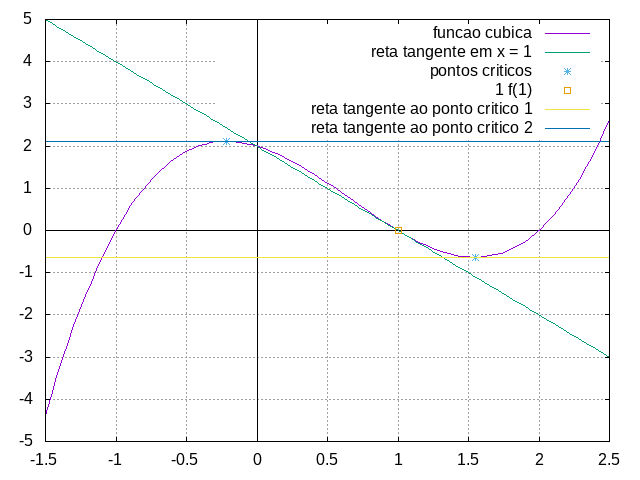
\includegraphics[scale=0.7]{exercicio1part.png}
        \caption{Exercício 1}
        \label{img:Exercício 1}
    \end{figure}
    
    \subsection*{Exercício 2}
    \hspace{1cm}Para o exercício 2 não nos é fornecido uma função pronta, porém, nos é dado um ponto conhecido da função e sua derivada. Com isso podemos estimar pontos dessa curva. Para calcular os pontos eu criei um algoritmo em Python. Segue abaixo o algoritmo:
    \lstinputlisting[language=python]{estimarpts.py}
    \hspace{1cm}Note que, foi utilizado a derivada da função e foi calculado os pontos a partir do ponto dado $f(0) = 1$ e foram calculadas 100 iterações para cada parte(negativa e positiva) com o valor de h = 0.05. Note ainda que, o algoritmo gera 2 arquivos diferentes, onde um arquivo é composto pelos pontos negativos e o outro pelos pontos positivos.\newline
    \hspace*{1cm}Com isso podemos agora plotar nosso gráfico gerado pelos pontos com o comando "plot "pontos negativos.pts" with lp, "pontos positivos.pts" with lp, x*cos(x) + 1".
    Segue o gráfico abaixo:\newline
    \begin{figure}[!h]
       \centering % Centraliza a imagem
        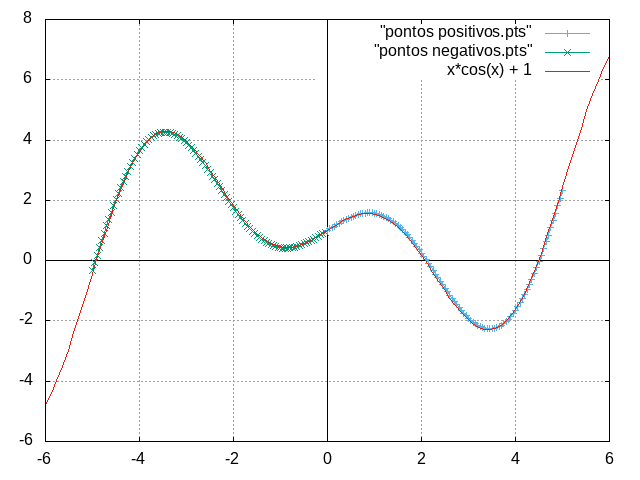
\includegraphics[scale=0.6]{exercicio2.png}
        \caption{Exercício 2 parte 1}
        \label{img:Exercício 2 parte 1}
    \end{figure}
    \newline \hspace*{1cm}Seguindo com a tarefa, o algoritmo a seguir foi criado para aplicarmos a aproximação da série de Taylor: 
    \lstinputlisting[language=python]{serieTaylor.py}
    \hspace{1cm}Esse algoritmo calcula o resultado das K-ésimas derivadas da função, onde o k nesse caso foi até 9. O algoritmo gerou as seguintes saídas: 1, 0, -3, 0, 5, -7, 0, 9.
    Agora, para calcularmos a aproximação da série de Taylor precisamos pegar esses valores acima e aplicar na fórmula $$\sum_{n=0}^{k=9} \frac{f^n(0)}{n!} x^n$$
    \hspace{1cm}Com isso temos a seguinte função: $f(x) = 1 + x - \frac{3}{6}x^3 + \frac{5}{120}x^5 - \frac{7}{5040}x^7 + \frac{9}{362880}x^9$.
    Plotando essa função no gnuplot temos:
    \begin{figure}[!h]
       \centering % Centraliza a imagem
        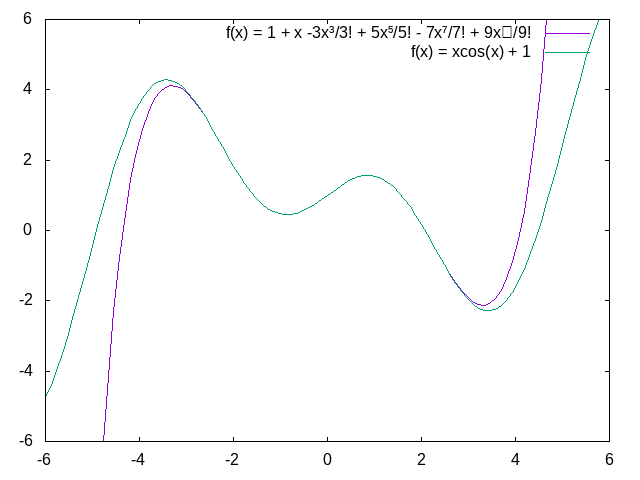
\includegraphics[scale=0.71]{exercicio2part2.png}
        \caption{Exercício 2 parte 2}
        \label{img:Exercício 2 parte 2}
    \end{figure}
    
\section*{Conclusão}
\hspace{1cm}A tarefa feita tinha por finalidade a plotagem das funções apresentadas na tarefa para que seja possível o aprendizado e aprofundamento das técnicas utilizadas para criação de gráficos elaborados para nossa visualização ou para a inserção em documentos, apresentações em slides ou etc. Além disso, a utilização de conceitos e aprendizados utilizados em matérias prévias como cálculo 1, para que fixemos as técnicas aprendidas dessa ferramenta de plotagem de gráficos chamada GNUPLOT.

\end{document}

